\section{Mappa e sue funzionalità}
La pagina della mappa è stata la sezione dell'applicazione più difficile da
implementare, perchè al suo interno risiedono numerosi servizi e funzioni che
hanno richiesto diverso tempo per essere sviluppati e inoltre è stato necessario
documentarsi per capire come utilizzare le API che la pagina utilizza.

\subsection{Scelta del servizio API}
In un primo momento si è pensato di utilizzare il servizio mappe di Google Maps
che, oltre ad essere uno dei più efficienti e meglio documentati, è anche
implementabile facilmente. Il problema è nato nel momento in cui Google ha
deciso di cambiare le proprie politiche di utilizzo delle API verso la fine del
2018. Prima di quel momento, sotto a un certo numero di richieste al servizio di
geolocalizzazione il programmatore poteva usare liberamente il codice e senza
necessità di registrazione, ma in seguito l'azienda di Mountain View ha deciso
che chiunque volesse utilizzare il proprio servizio mappe dovesse prima
registrare un proprio account ed inserire una carta di credito che eventualmente
pagasse mensilmente le risorse di cui si è fatto uso. Questo scenario ha portato
a prendere in cosiderazione altri gestori di mappe. La scelta è ricaduta su
MapBox, azienda emergente nel proprio campo. Il servizio era gratuito e permetteva
un agevole utilizzo senza registrazione ma il problema era formato
dall'implementazione vera e propria. Al contrario di Google, non esiste un
pacchetto software che implementi il codice MapBox e quindi era necessario fare
uso di richieste http tramite valori codificati all'interno di lunghi url.
Inoltre la fluidità della mappa non rispettava le direttive del committente
dott. Marco Aceti, spesso a seguito di un rapido movimento delle dita per
spostarsi in un'altra zona della mappa la schermata rimaneva per qualche secondo
completamente grigia, rendendo l'esperienza di utilizzo sicuramente peggiore.
Nel seguito, tra Gennaio e Febbraio 2019 è stata rilasciata la prima versione
ufficiale di Flutter (versione 1.0.0) e tra le tante novità spiccava la presenza
di un widget particolare, chiamato GoogleMap. Semplificando notevolmente
l'utilizzo delle mappe, tale widget presenta ottime prestazioni e facilità di
implementazione. Si è quindi deciso di dedicare del tempo nell'apprendere ogni
aspetto delle politiche di utilizzo delle API di Google, capendo quindi che,
facendo un numero di richieste minore di una soglia stabilita, non è necessario
pagare nulla, anche se si è registrata una carta di credito. Quindi la scelta è
ricaduta sulle API di Google e si è importato nel progetto il pacchetto
\verb|googlemap|.

\subsection{MapPage}
Dopo che l'utente ha eseguito correttamente la procedura di login o ha aperto
l'applicazione in caso di autoidentificazione con mantenimento dello stato della
registrazione, viene mostrata la MapPage. In alto è presente un'AppBar che 
mostra il titolo eBike-Recharge, in basso è presente una TabBar che permette di
navigare tra le pagine dell'app. Tra le due, a tutto schermo, viene mostrata la
mappa con al centro la posizione attuale dell'utente. Quest'ultima può essere di
diversi tipi a seconda delle preferenze indicate nella pagina profilo
dell'utilizzatore. In particolare si può scegliere tra \textit{Normale}, cioè la
classica modalità di visualizzazione di mappe che viene mostrata di default
sull'app Google Maps, \textit{Rilievo}, dove è presente l'altitudine delle
montagne indicata con diversi colori in base all'altezza, mancando però
di indicare i nomi di edifici importanti, negozi o imprese, \textit{Satellite},
che mostra con una serie di foto satellitari i luoghi indicati dall'alto, in
modo da vedere realmente il percorso che si deve intraprendere
per raggiungere la propria destinazione, e \textit{Ibrida}, che può essere
considerata l'unione di Satellitare e Normale, poichè oltre a presentare
l'altitudine mostra anche i nomi dei luoghi di maggior importanza della zona
visualizzata.

\begin{figure}[h!]
    \centering
    \begin{subfigure}{0.33\linewidth}
        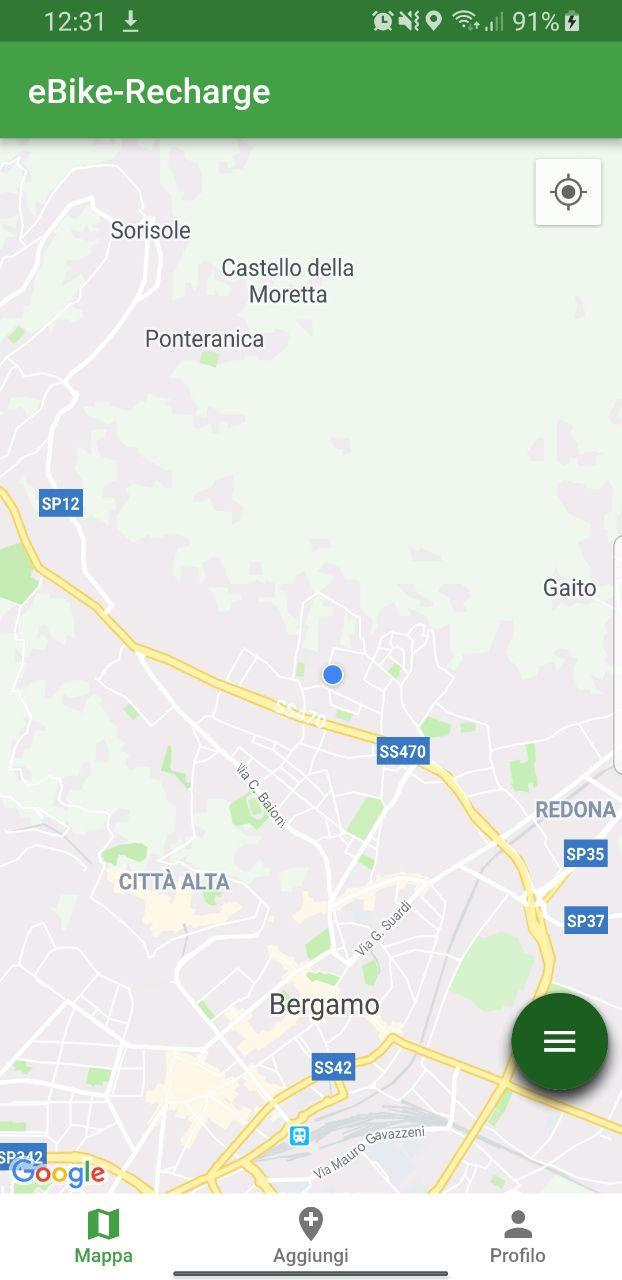
\includegraphics[width=\linewidth, height=9cm]{MapNormale.jpg}
        \caption{Normale}
    \end{subfigure}
    \begin{subfigure}{0.33\linewidth}
        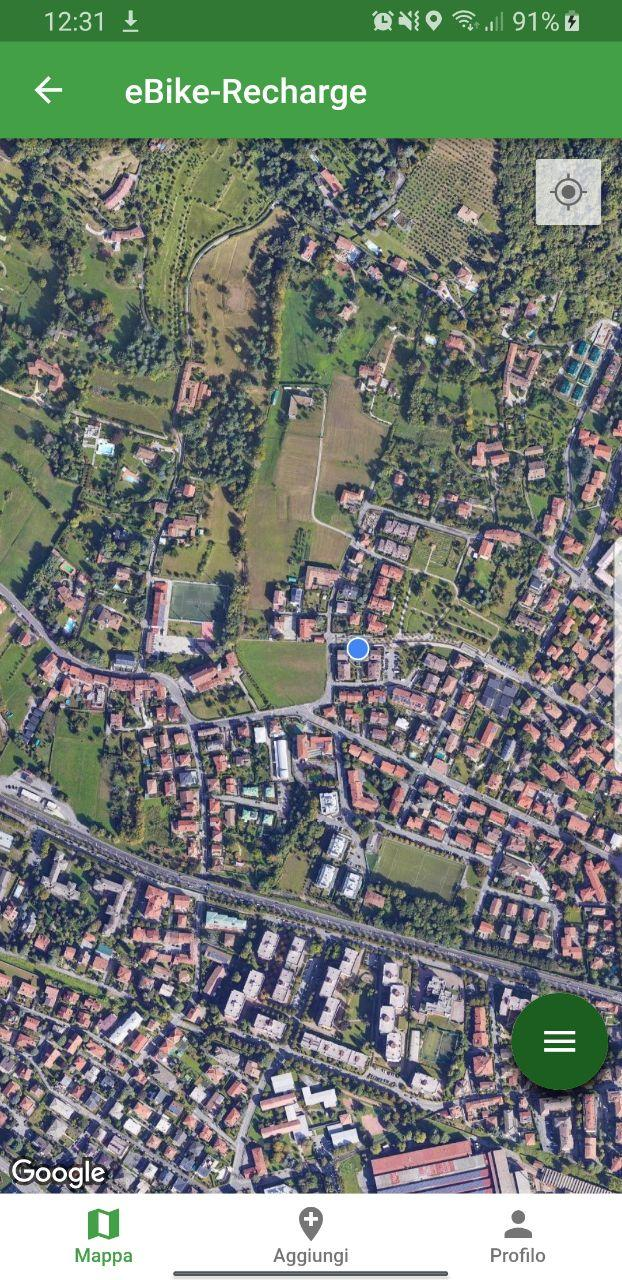
\includegraphics[width=\linewidth, height=9cm]{MapSatellite.jpg}
        \caption{Satellite}
    \end{subfigure}
    \begin{subfigure}{0.33\linewidth}
        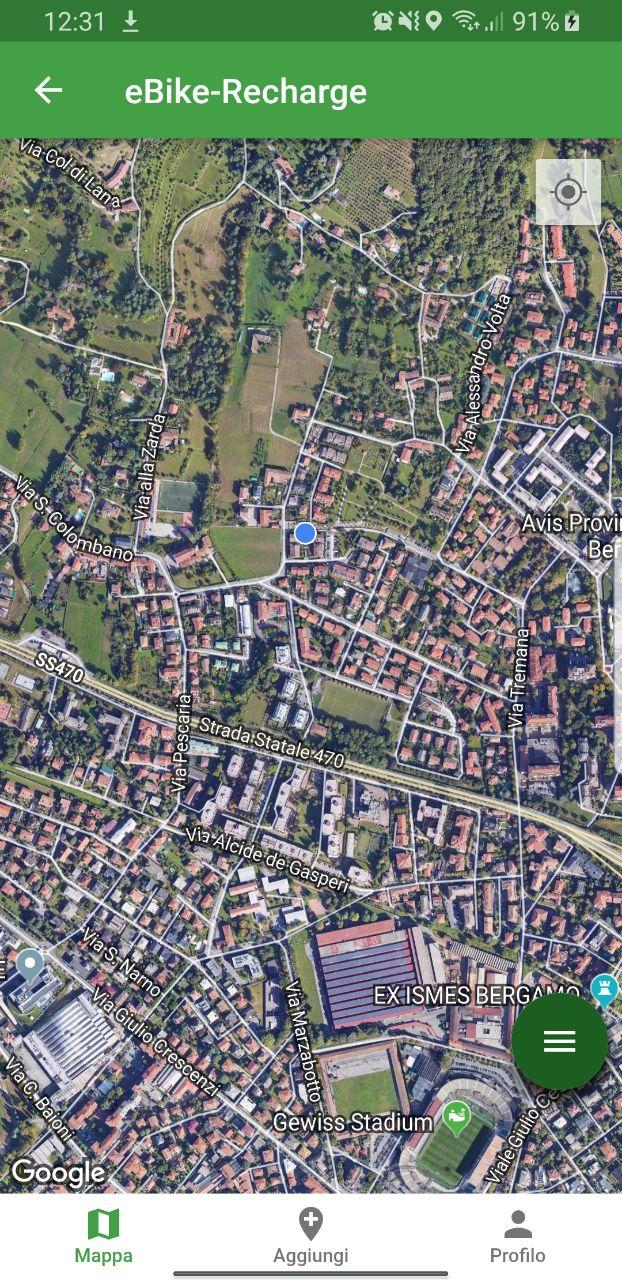
\includegraphics[width=\linewidth, height=9cm]{MapIbrida.jpg}
        \caption{Ibrida}
    \end{subfigure}
    \begin{subfigure}{0.33\linewidth}
        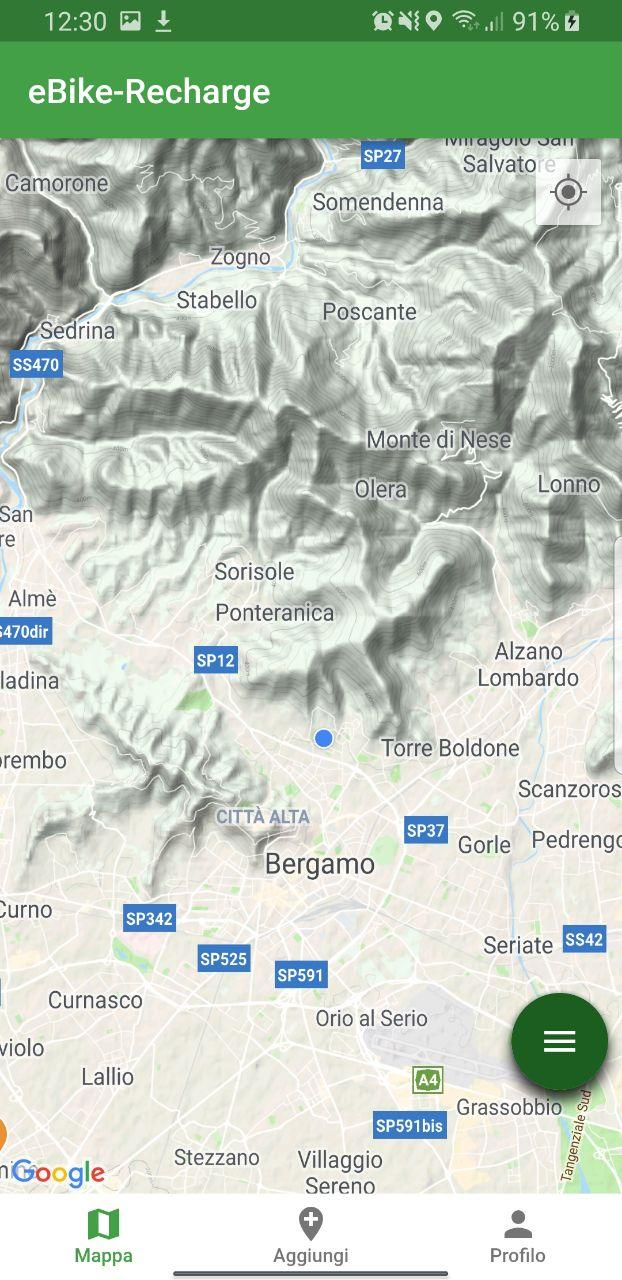
\includegraphics[width=\linewidth, height=9cm]{MapRilievo.jpg}
        \caption{Rilievo}
    \end{subfigure}
    \caption{I quattro tipi di mappa selezionabili nella pagina profilo}
    \label{TipoMappa}
\end{figure} 

Grazie al pacchetto googlemap di flutter si è riusciti a implementare un oggetto
GoogleMap (che verrà descritto in un successivo paragrafo) con cui è molto
facile interagire. In particolare, l'utente può aumentare o diminuire lo zoom
della mappa con i classici gesti di allontanamento o avvicinamento delle dita, e
può spostarsi in diverse zona semplicemente trascinando verso la direzione
desiderata. Con una buona o anche solo media connessione internet i tempi di
latenza sono pressochè nulli, così che non si riesca a vedere i riquadri grigi
che il widget crea nel momento in cui si cambia direzione e che dovranno essere
riempiti con le nuove località. Questi ultimi sono pienamente visibili nel
momento in cui non si disponga di una connessione adeguata, condizione che si
verifica sempre più di rado negli ultimi tempi. 


\subsection{Funzionalità}
Nelle immagini precedenti si è forse notato un pulsante nella parte inferiore
dello schermo verso destra. Se toccato (figura \ref{4puls}), quest'ultimo mostra una serie di
pulsanti con diverse funzionalità. 
\begin{figure}
    \centering
    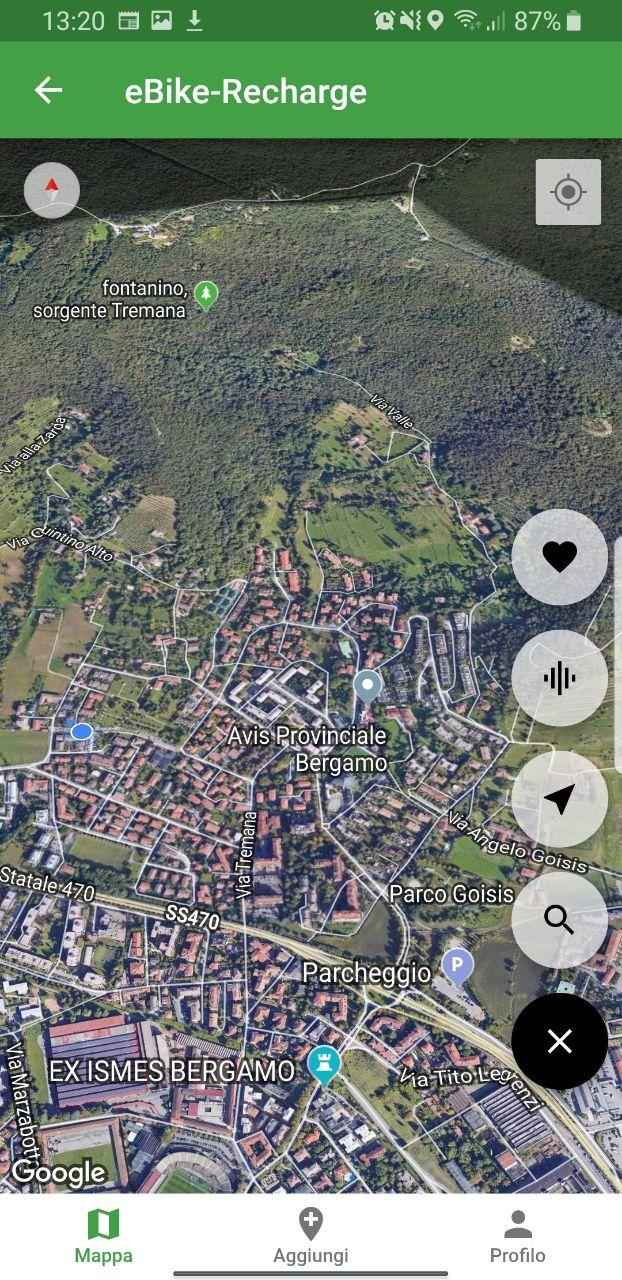
\includegraphics[width=7cm]{MapFun.jpg}
    \caption{Premuto il pulsante, vengono mostrati i 4 FloatingActionButton e il quinto (con la X) per tornare indietro}
    \label{4puls}
\end{figure}
Il primo è un'icona a forma di cuore e,
interagendo con esso, viene mostrato un BottomSheet (spiegato nel secondo
capitolo, Flutter) che mostra una Card (una piccola scheda con titolo e icona)
con le stazioni di ricarica preferite dall'utente. Per esprimere la propria
preferenza per una stazione è necessario entrare nella scheda di quest'ultima e
selezionare il cuore presente in alto a destra. \\
Il secondo pulsante ha la funzione di filtro e al tempo stesso di legenda.
Premendolo, viene mostrata a schermo una AlertDialog (fig. \ref{filtro}) che indica quali
tipologie di stazioni si desidera cercare. Sulla destra sono presenti dei Button
di tipo check (che possono essere True o False): se si vede la casella spuntata
allora si vedra la relativa tipologia sulla mappa, se tale casella è vuota
allora la mappa verrà filtrata e non sarà possibile cercare tutte le stazioni di
quel tipo. \\
Il terzo pulsante mostra un'icona con la classica freccia indicante la
navigazione e, se premuto, fa apparire un BottomSheet con Card contenente le
dieci stazioni più vicine alla posizione attuale dell'utente. Come per tutte le
Card anche nelle altre funzionalità, è possibile definire un'azione in seguito
al tocco della scheda. In seguito all'interazione dell'utilizzatore con una
specifica Card, la mappa ruota e cambia il proprio centro mostrando l'icona
indicante quella stazione che si è toccata. In questo modo l'utente risparmia
tempo poichè viene direttamente condotto alla stazione di interesse.
\begin{figure}[h!]
    \centering
    \begin{subfigure}{0.3\linewidth}
        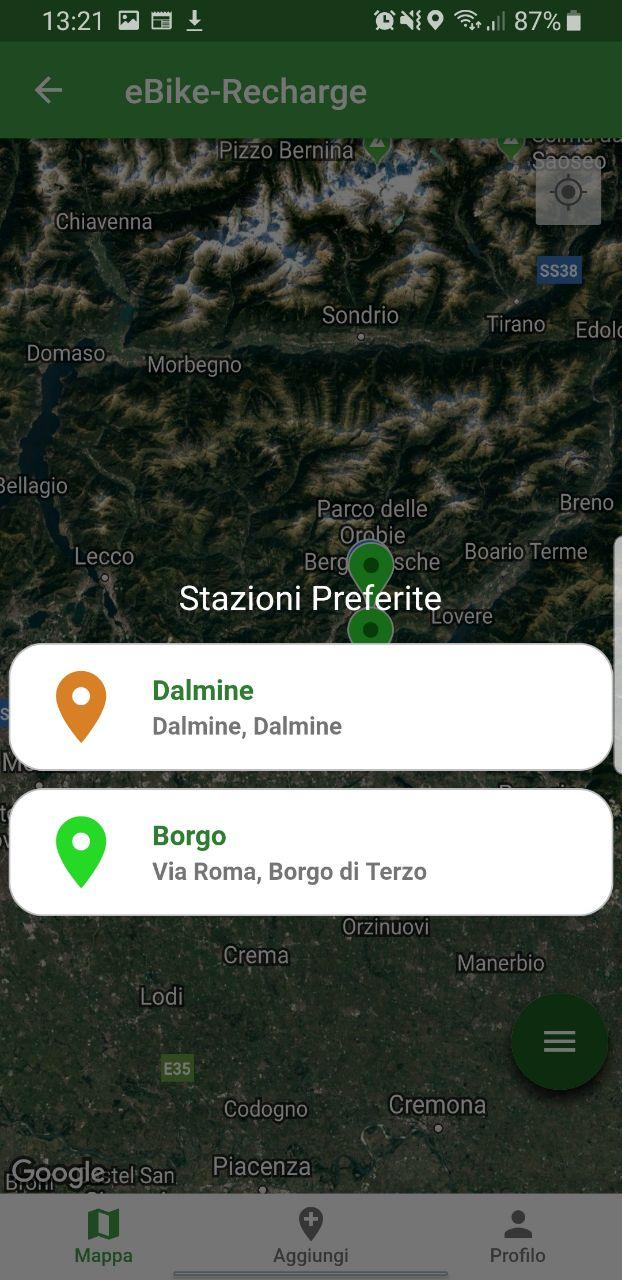
\includegraphics[width=\linewidth, height=9cm]{MapFunFavourite.jpg}
        \caption{Preferiti}
    \end{subfigure}
    \begin{subfigure}{0.3\linewidth}
        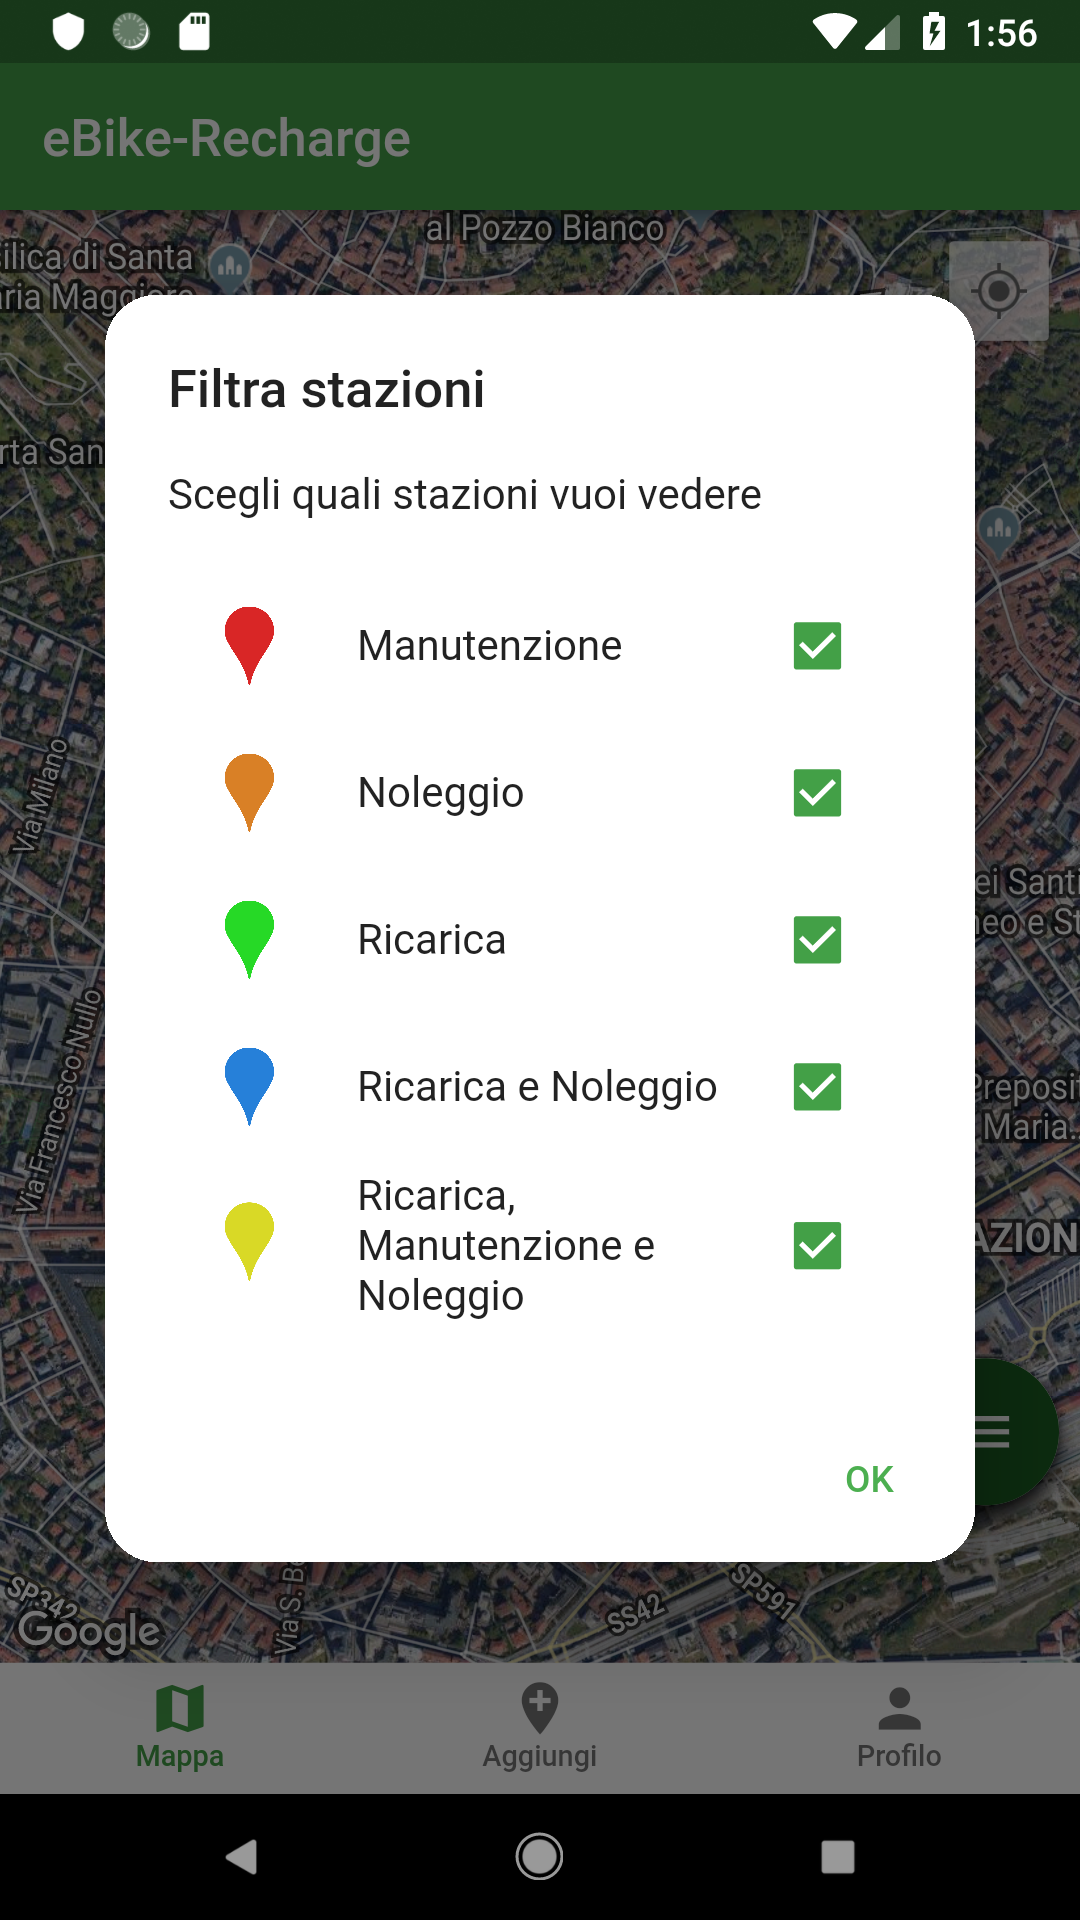
\includegraphics[width=\linewidth, height=9cm]{MapFunFilter.png}
        \caption{Filtro e Legenda}
        \label{filtro}
    \end{subfigure}
    \begin{subfigure}{0.3\linewidth}
        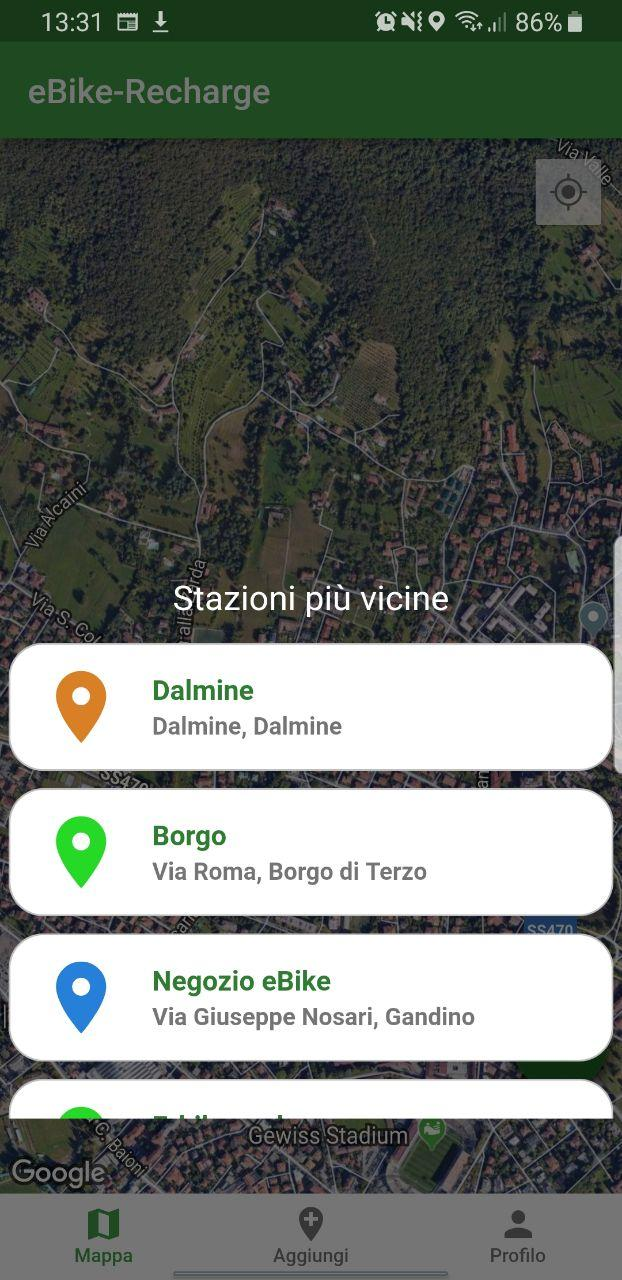
\includegraphics[width=\linewidth, height=9cm]{MapFunNearest.jpg}
        \caption{Stazioni più vicine}
    \end{subfigure}
    \caption{}
\end{figure}

L'ultimo pulsante è accompagnato da un'icona rappresentante una lente di
ingrandimento, simbolo universale di ricerca. Premendolo, in alto sullo schermo
appare un TextField con impresso la frase "Cerca Indirizzo". L'utente è quindi
invitato a digitare la via o la località che desidera vedere. Mentre si forma la
scritta, grazie al servizio API Google Places l'app è in grado di mostrare
diverse Card a schermo con suggerimenti, fungendo quindi da auto-completamento.
Se l'utente clicca su una di queste sezioni viene richiamata la stessa funzione
delle Card prima mostrata: la mappa cambia centro e porta l'utente nella via
desiderata. Questo servizio costa una frazione di centesimo per ogni singola
chiamata alla funzione di auto-completamento. Si è quindi deciso di introdurre
un limite mensile al numero di volte che l'app può far uso di questa API, in
corrispondenza del numero massimo di chiamate che si possono fare senza dover
pagare direttamente Google.
\begin{figure}[h!]
    \centering
    \begin{subfigure}{0.33\linewidth}
        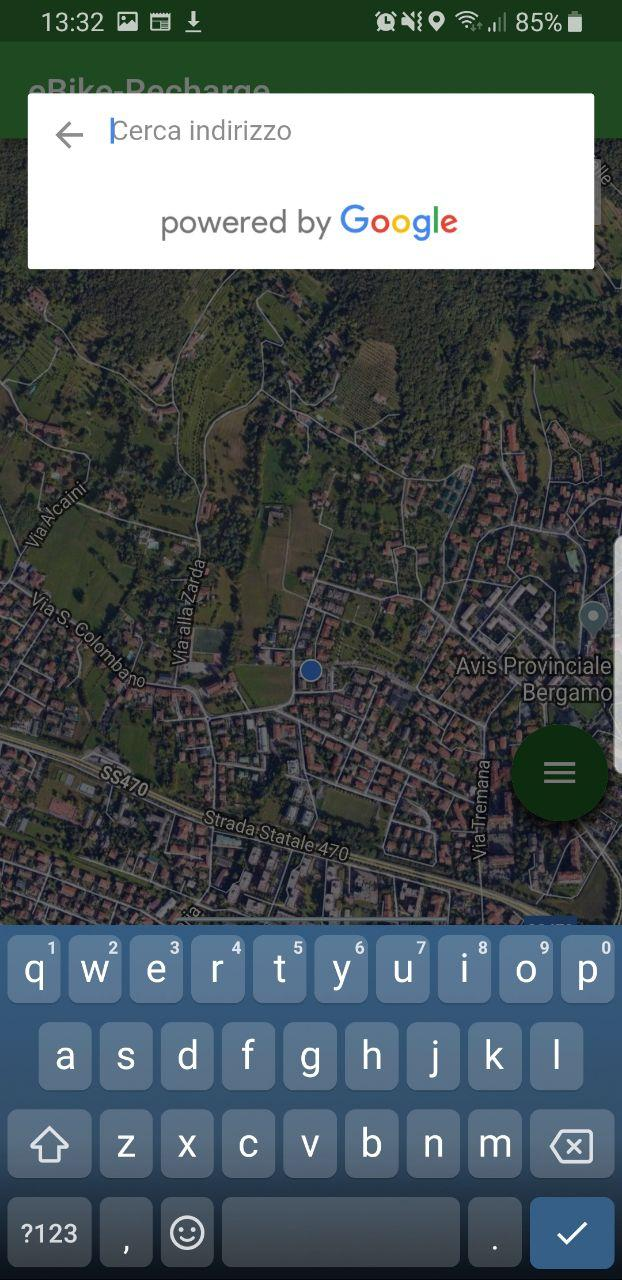
\includegraphics[width=\linewidth, height=9cm]{MapFunSearch1.jpg}
    \end{subfigure}
    \begin{subfigure}{0.33\linewidth}
        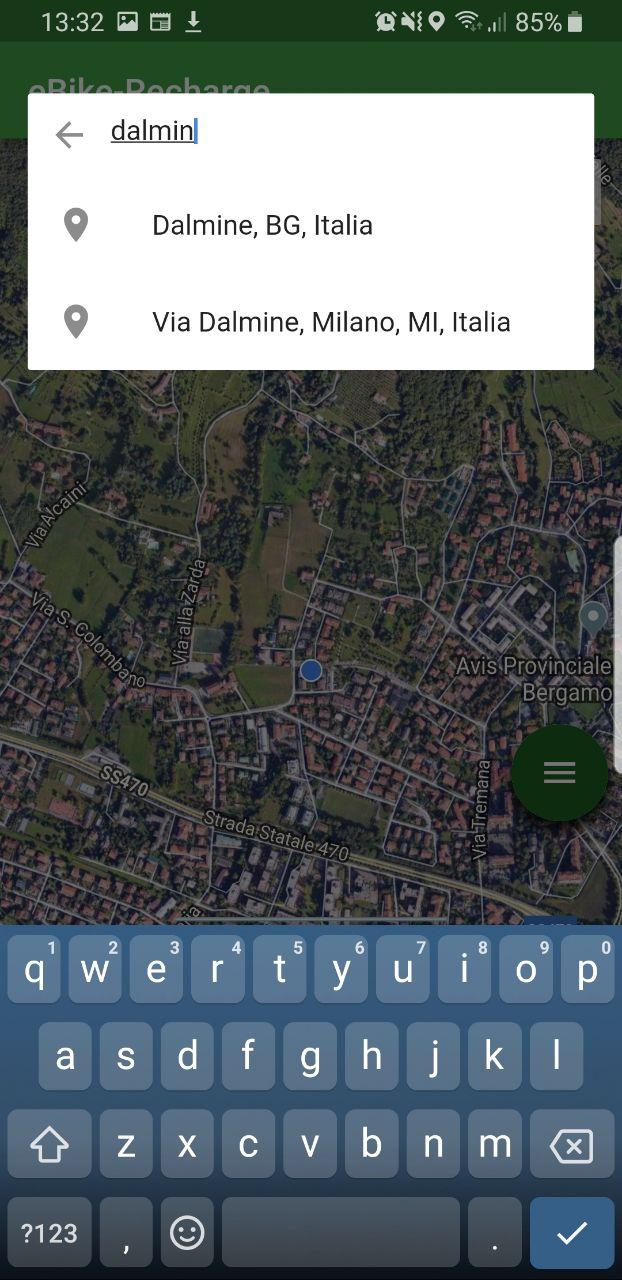
\includegraphics[width=\linewidth, height=9cm]{MapFunSearch2.jpg}
    \end{subfigure}
    \caption{La funzione di ricerca e autocompletamento dell'API Google Places}
\end{figure}

\subsection{Aggiungere una Stazione}